\documentclass{standalone}
\usepackage{tikz}
\usetikzlibrary{patterns, positioning}


\begin{document}
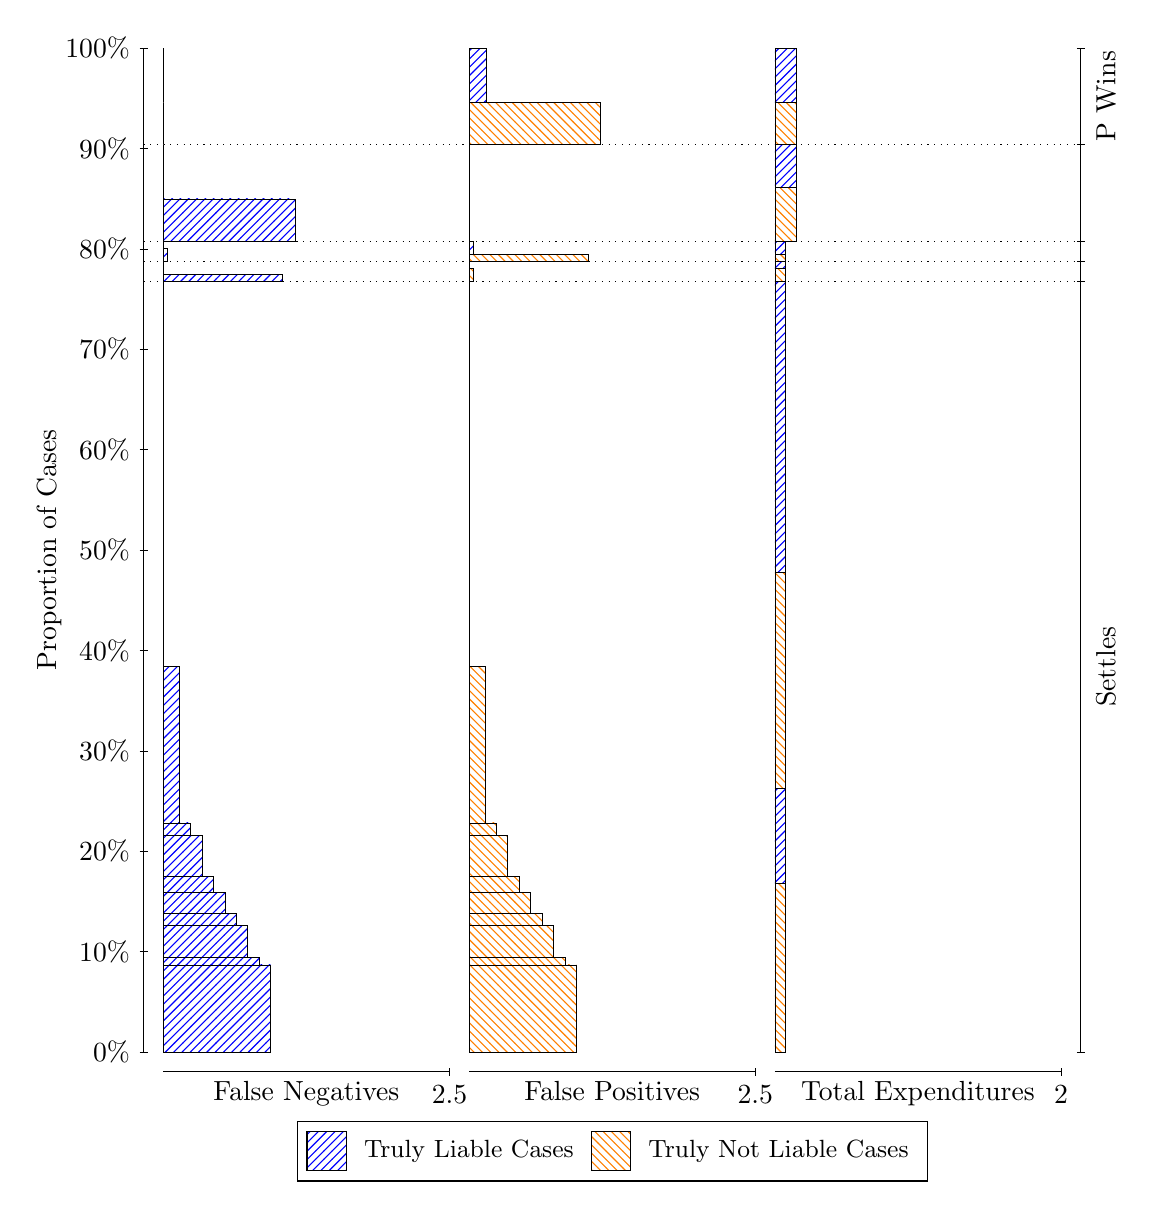
\begin{tikzpicture}
\draw[black, very thin] (1.5,1.75) -- (1.5,14.5);
\node[rotate=90, text=black, anchor=center] at (0.3, 8.125) {Proportion of Cases};
\draw[black, very thin] (1.45,1.75) -- (1.55,1.75);
\node[text=black, anchor=east] at (1.45, 1.75) {0\%};
\draw[black, very thin] (1.45,3.025) -- (1.55,3.025);
\node[text=black, anchor=east] at (1.45, 3.025) {10\%};
\draw[black, very thin] (1.45,4.3) -- (1.55,4.3);
\node[text=black, anchor=east] at (1.45, 4.3) {20\%};
\draw[black, very thin] (1.45,5.575) -- (1.55,5.575);
\node[text=black, anchor=east] at (1.45, 5.575) {30\%};
\draw[black, very thin] (1.45,6.85) -- (1.55,6.85);
\node[text=black, anchor=east] at (1.45, 6.85) {40\%};
\draw[black, very thin] (1.45,8.125) -- (1.55,8.125);
\node[text=black, anchor=east] at (1.45, 8.125) {50\%};
\draw[black, very thin] (1.45,9.4) -- (1.55,9.4);
\node[text=black, anchor=east] at (1.45, 9.4) {60\%};
\draw[black, very thin] (1.45,10.675) -- (1.55,10.675);
\node[text=black, anchor=east] at (1.45, 10.675) {70\%};
\draw[black, very thin] (1.45,11.95) -- (1.55,11.95);
\node[text=black, anchor=east] at (1.45, 11.95) {80\%};
\draw[black, very thin] (1.45,13.225) -- (1.55,13.225);
\node[text=black, anchor=east] at (1.45, 13.225) {90\%};
\draw[black, very thin] (1.45,14.5) -- (1.55,14.5);
\node[text=black, anchor=east] at (1.45, 14.5) {100\%};

\draw[black, very thin] (13.4,1.75) -- (13.4,14.5);
\draw[black, very thin] (13.35,1.75) -- (13.45,1.75);
\node[anchor=west] at (13.35, 1.75) {};
\draw[black, very thin] (13.35,11.538) -- (13.45,11.538);
\node[anchor=west] at (13.35, 11.538) {};
\draw[black, very thin] (13.35,11.792) -- (13.45,11.792);
\node[anchor=west] at (13.35, 11.792) {};
\draw[black, very thin] (13.35,12.046) -- (13.45,12.046);
\node[anchor=west] at (13.35, 12.046) {};
\draw[black, very thin] (13.35,13.273) -- (13.45,13.273);
\node[anchor=west] at (13.35, 13.273) {};
\draw[black, very thin] (13.35,14.5) -- (13.45,14.5);
\node[anchor=west] at (13.35, 14.5) {};

\draw[black, very thin, pattern color=blue, pattern=north east lines] (1.75,1.75) rectangle (3.1125,2.8556);
\draw[black, very thin, pattern color=blue, pattern=north east lines] (1.75,2.8556) rectangle (2.9672,2.9478);
\draw[black, very thin, pattern color=blue, pattern=north east lines] (1.75,2.9478) rectangle (2.8218,3.3568);
\draw[black, very thin, pattern color=blue, pattern=north east lines] (1.75,3.3568) rectangle (2.6765,3.5142);
\draw[black, very thin, pattern color=blue, pattern=north east lines] (1.75,3.5142) rectangle (2.5312,3.7772);
\draw[black, very thin, pattern color=blue, pattern=north east lines] (1.75,3.7772) rectangle (2.3858,3.9761);
\draw[black, very thin, pattern color=blue, pattern=north east lines] (1.75,3.9761) rectangle (2.2405,4.4991);
\draw[black, very thin, pattern color=blue, pattern=north east lines] (1.75,4.4991) rectangle (2.0952,4.66);
\draw[black, very thin, pattern color=blue, pattern=north east lines] (1.75,4.66) rectangle (1.9498,6.6439);
\draw[black, very thin, pattern color=orange, pattern=north west lines] (1.75,6.6439) rectangle (1.75,11.538);
\draw[black, very thin, pattern color=blue, pattern=north east lines] (1.75,11.538) rectangle (3.2578,11.629);
\draw[black, very thin, pattern color=orange, pattern=north west lines] (1.75,11.629) rectangle (1.75,11.792);
\draw[black, very thin, pattern color=blue, pattern=north east lines] (1.75,11.792) rectangle (1.8045,11.955);
\draw[black, very thin, pattern color=orange, pattern=north west lines] (1.75,11.955) rectangle (1.75,12.046);
\draw[black, very thin, pattern color=blue, pattern=north east lines] (1.75,12.046) rectangle (3.4213,12.584);
\draw[black, very thin, pattern color=orange, pattern=north west lines] (1.75,12.584) rectangle (1.75,13.273);
\draw[black, very thin, pattern color=orange, pattern=north west lines] (1.75,13.273) rectangle (1.75,13.811);
\draw[black, very thin, pattern color=blue, pattern=north east lines] (1.75,13.811) rectangle (1.75,14.5);
\draw[black, very thin, pattern color=orange, pattern=north west lines] (5.6333,1.75) rectangle (6.9958,2.8555);
\draw[black, very thin, pattern color=orange, pattern=north west lines] (5.6333,2.8555) rectangle (6.8505,2.9477);
\draw[black, very thin, pattern color=orange, pattern=north west lines] (5.6333,2.9477) rectangle (6.7052,3.3567);
\draw[black, very thin, pattern color=orange, pattern=north west lines] (5.6333,3.3567) rectangle (6.5598,3.5141);
\draw[black, very thin, pattern color=orange, pattern=north west lines] (5.6333,3.5141) rectangle (6.4145,3.7772);
\draw[black, very thin, pattern color=orange, pattern=north west lines] (5.6333,3.7772) rectangle (6.2692,3.9761);
\draw[black, very thin, pattern color=orange, pattern=north west lines] (5.6333,3.9761) rectangle (6.1238,4.499);
\draw[black, very thin, pattern color=orange, pattern=north west lines] (5.6333,4.499) rectangle (5.9785,4.66);
\draw[black, very thin, pattern color=orange, pattern=north west lines] (5.6333,4.66) rectangle (5.8332,6.644);
\draw[black, very thin, pattern color=blue, pattern=north east lines] (5.6333,6.644) rectangle (5.6333,11.538);
\draw[black, very thin, pattern color=orange, pattern=north west lines] (5.6333,11.538) rectangle (5.6878,11.701);
\draw[black, very thin, pattern color=blue, pattern=north east lines] (5.6333,11.701) rectangle (5.6333,11.792);
\draw[black, very thin, pattern color=orange, pattern=north west lines] (5.6333,11.792) rectangle (7.1412,11.883);
\draw[black, very thin, pattern color=blue, pattern=north east lines] (5.6333,11.883) rectangle (5.6878,12.046);
\draw[black, very thin, pattern color=orange, pattern=north west lines] (5.6333,12.046) rectangle (5.6333,12.735);
\draw[black, very thin, pattern color=blue, pattern=north east lines] (5.6333,12.735) rectangle (5.6333,13.273);
\draw[black, very thin, pattern color=orange, pattern=north west lines] (5.6333,13.273) rectangle (7.3047,13.811);
\draw[black, very thin, pattern color=blue, pattern=north east lines] (5.6333,13.811) rectangle (5.8513,14.5);
\draw[black, very thin, pattern color=orange, pattern=north west lines] (9.5167,1.75) rectangle (9.6529,3.8949);
\draw[black, very thin, pattern color=blue, pattern=north east lines] (9.5167,3.8949) rectangle (9.6529,5.0927);
\draw[black, very thin, pattern color=orange, pattern=north west lines] (9.5167,5.0927) rectangle (9.6529,7.8417);
\draw[black, very thin, pattern color=blue, pattern=north east lines] (9.5167,7.8417) rectangle (9.6529,11.538);
\draw[black, very thin, pattern color=orange, pattern=north west lines] (9.5167,11.538) rectangle (9.6529,11.701);
\draw[black, very thin, pattern color=blue, pattern=north east lines] (9.5167,11.701) rectangle (9.6529,11.792);
\draw[black, very thin, pattern color=orange, pattern=north west lines] (9.5167,11.792) rectangle (9.6529,11.883);
\draw[black, very thin, pattern color=blue, pattern=north east lines] (9.5167,11.883) rectangle (9.6529,12.046);
\draw[black, very thin, pattern color=orange, pattern=north west lines] (9.5167,12.046) rectangle (9.7892,12.735);
\draw[black, very thin, pattern color=blue, pattern=north east lines] (9.5167,12.735) rectangle (9.7892,13.273);
\draw[black, very thin, pattern color=orange, pattern=north west lines] (9.5167,13.273) rectangle (9.7892,13.811);
\draw[black, very thin, pattern color=blue, pattern=north east lines] (9.5167,13.811) rectangle (9.7892,14.5);
\draw[black, dotted] (1.5,11.538) -- (13.4,11.538);
\draw[black, dotted] (1.5,11.792) -- (13.4,11.792);
\draw[black, dotted] (1.5,12.046) -- (13.4,12.046);
\draw[black, dotted] (1.5,13.273) -- (13.4,13.273);
\draw[black, very thin] (1.75,1.5) -- (5.3833,1.5);
\node[text=black, anchor=north] at (3.5667, 1.5) {False Negatives};
\draw[black, very thin] (5.3833,1.45) -- (5.3833,1.55);
\node[text=black, anchor=north] at (5.3833, 1.45) {2.5};

\draw[black, very thin] (5.6333,1.5) -- (9.2667,1.5);
\node[text=black, anchor=north] at (7.45, 1.5) {False Positives};
\draw[black, very thin] (9.2667,1.45) -- (9.2667,1.55);
\node[text=black, anchor=north] at (9.2667, 1.45) {2.5};

\draw[black, very thin] (9.5167,1.5) -- (13.15,1.5);
\node[text=black, anchor=north] at (11.333, 1.5) {Total Expenditures};
\draw[black, very thin] (13.15,1.45) -- (13.15,1.55);
\node[text=black, anchor=north] at (13.15, 1.45) {2};

\node[text=black, centered, rotate=90] at (13.72, 6.6439) {Settles};



\node[text=black, centered, rotate=90] at (13.72, 13.887) {P Wins};

\draw (7.449999999999999,1.5) node[draw=none] (baseCoordinate) {};
\begin{scope}[align=center]
        \matrix[scale=0.5, draw=black, below=0.5cm of baseCoordinate, nodes={draw}, column sep=0.1cm]{
            \node[rectangle, draw, minimum width=0.5cm, minimum height=0.5cm, pattern color=blue, pattern=north east lines] {}; &
            \node[draw=none, font=\small, text=black] (B) {Truly Liable Cases}; &
            \node[rectangle, draw, minimum width=0.5cm, minimum height=0.5cm, pattern color=orange, pattern=north west lines] {}; &
            \node[draw=none, font=\small, text=black] (B) {Truly Not Liable Cases}; \\
            };
\end{scope}

\end{tikzpicture}
\end{document}